\documentclass{beamer}

\mode<presentation>
{
   \usetheme{EEng}
%   \usetheme{Warsaw}
  \setbeamercovered{transparent}
  \setbeamercolor{background canvas}{bg=black!0}
}

\usepackage{enumerate}
\usepackage{array}
\usepackage{graphics}
\usepackage{ucs}
\usepackage[utf8x]{inputenc}
\usepackage[english]{babel}
\usepackage{amsmath, amsthm, amssymb}
\usepackage{amsmath}
\usepackage{amsfonts}
\usepackage{xcolor}
\usepackage{pgf}
\usepackage{hyperref}
\usepackage{url}
\usepackage{multicol}   % add-on
\usepackage{boxedminipage} 
\usepackage{indentfirst}   % add-on
\usepackage{float}
\usepackage[all]{xypic}
\usepackage{listings}
\usepackage{verbatim}
\usepackage{boxedminipage}

% % % inicio do listings e ref
\definecolor{darkblue}{rgb}{0,0,0.6}
\definecolor{gray_ulisses}{gray}{0.55}
\definecolor{castanho_ulisses}{rgb}{0.71,0.33,0.14}
\definecolor{preto_ulisses}{rgb}{0.41,0.20,0.04}
\definecolor{green_ulises}{rgb}{0.2,0.75,0}

\hypersetup{
    a4paper,
    pdftex,
    bookmarks,
    colorlinks,
    citecolor=darkblue,
    linkcolor=darkblue,
    urlcolor=darkblue,
    filecolor=darkblue
}

\lstdefinelanguage{perl_u} {
       basicstyle=\ttfamily\tiny,
       showstringspaces=false,
       breaklines=true,
       numbers=left,
       numberstyle=\tiny,
       numberblanklines=true,
       showspaces=false,
       showtabs=false
}
% % % fim do listings e ref

\title{GD::Graph - Graph Plotting Module}
\author{José Pedro Silva \and
Pedro Faria \and
Ulisses Costa
}

\date{\today}
\institute{Engenharia de Linguagens\\
Projecto integrado
}

\AtBeginSubsection[] {
  \begin{frame}<beamer>
    \frametitle{Index}
    \scriptsize{\tableofcontents[currentsection,currentsubsection]}
  \end{frame}
}

\AtBeginSection[] {
  \begin{frame}<beamer>
    \frametitle{Index}
    \scriptsize{\tableofcontents[currentsection]}
  \end{frame}
}
\begin{document}
\begin{frame}
   \titlepage
\end{frame}

\begin{frame} \frametitle{Description}
GD::Graph is a perl5 module to create charts using the GD module. The following classes for graphs with axes are defined:
\begin{description}
\item[GD::Graph::lines] Create a line chart.
\item[GD::Graph::bars] Create a bar chart with vertical or horizontal bars.
\item[GD::Graph::linespoints] Combination of lines and points.
\item[GD::Graph::area] Create a graph, representing the data as areas under a line.
\item[GD::Graph::pie] Create a pie chart.
\end{description}
\end{frame}

\begin{frame}[fragile] \frametitle{Bars}
\begin{lstlisting}[language=perl_u,breaklines=true]
sub plotPng {    
    my $fileName = shift;
    @data = ( ["1st","2nd","3rd","4th","5th","6th","7th", "8th", "9th"],
              [    1,    2,    5,    6,    3,  1.5,    1,     3,     4]
            );
    my $mygraph = GD::Graph::bars->new(600, 400);
    
    $mygraph->set (
        x_label       => "Contestant",
        y_label       => "Time",
        title         => "Times of the contestants",
        dclrs         =>  [ qw(gold red green) ],
    ) or warn $mygraph->error;

    my $myimage = $mygraph->plot(\@data) or warn $mygraph->error;
    
    open (IMG, '>' , $fileName);
    binmode IMG;
    print IMG $myimage->png;
    close (IMG);
}
\end{lstlisting}
\end{frame}

\begin{frame} \frametitle{Bars - Output}
\begin{figure}[htbp]
\begin{center}
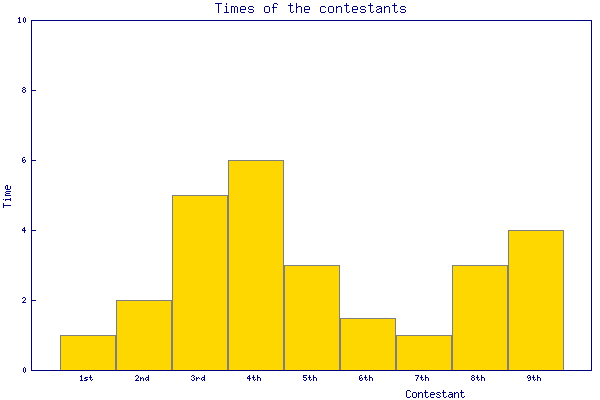
\includegraphics[width=0.9\textwidth]{image/1.png}
\end{center}
\end{figure}
\end{frame}

\begin{frame}[fragile] \frametitle{Pie}
\begin{lstlisting}[language=perl_u,breaklines=true]
sub plotPng {    
    my $fileName = shift;
    @data = ( ["1st","2nd","3rd","4th","5th","6th","7th", "8th", "9th"],
              [    1,    2,    5,    6,    3,  1.5,    1,     3,     4]
            );
    my $mygraph = GD::Graph::pie->new(600, 400);
    
    $mygraph->set (
        title         => "Times of the contestants",
        dclrs         =>  [ qw(gold red green) ],
    ) or warn $mygraph->error;

    my $myimage = $mygraph->plot(\@data) or warn $mygraph->error;
    
    open (IMG, '>' , $fileName);
    binmode IMG;
    print IMG $myimage->png;
    close (IMG);
}
\end{lstlisting}
\end{frame}

\begin{frame} \frametitle{Pie - Output}
\begin{figure}[htbp]
\begin{center}
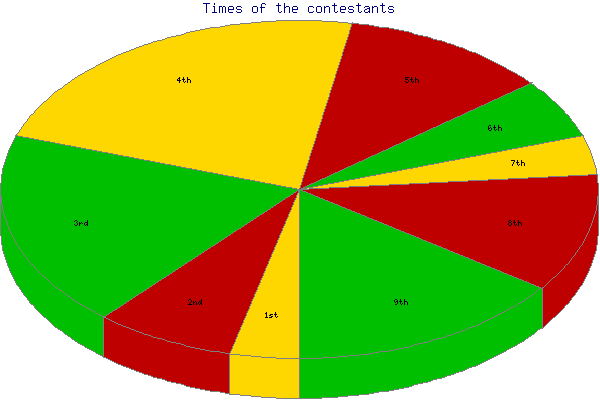
\includegraphics[width=0.9\textwidth]{image/2.png}
\end{center}
\end{figure}
\end{frame}

\begin{frame}[fragile] \frametitle{Line}
\begin{lstlisting}[language=perl_u,breaklines=true]
sub plotPng {    
    my $fileName = shift;
    @data = ( ["1st","2nd","3rd","4th","5th","6th","7th", "8th", "9th"],
              [    1,    2,    5,    6,    3,  1.5,    1,     3,     4]
            );
    my $mygraph = GD::Graph::area->new(600, 400);
    
    $mygraph->set (
        title         => "Times of the contestants",
        dclrs         =>  [ qw(gold red green) ],
    ) or warn $mygraph->error;

    my $myimage = $mygraph->plot(\@data) or warn $mygraph->error;
    
    open (IMG, '>' , $fileName);
    binmode IMG;
    print IMG $myimage->png;
    close (IMG);
}
\end{lstlisting}
\end{frame}

\begin{frame} \frametitle{Line - Output}
\begin{figure}[htbp]
\begin{center}
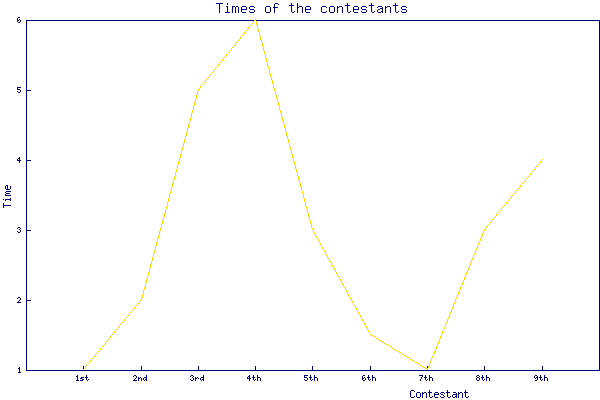
\includegraphics[width=0.9\textwidth]{image/lines.png}
\end{center}
\end{figure}
\end{frame}

\begin{frame}[fragile] \frametitle{Area}
\begin{lstlisting}[language=perl_u,breaklines=true]
sub plotPng {    
    my $fileName = shift;
    @data = ( ["1st","2nd","3rd","4th","5th","6th","7th", "8th", "9th"],
              [    1,    2,    5,    6,    3,  1.5,    1,     3,     4]
            );
    my $mygraph = GD::Graph::area->new(600, 400);
    
    $mygraph->set (
        title         => "Times of the contestants",
        dclrs         =>  [ qw(gold red green) ],
    ) or warn $mygraph->error;

    my $myimage = $mygraph->plot(\@data) or warn $mygraph->error;
    
    open (IMG, '>' , $fileName);
    binmode IMG;
    print IMG $myimage->png;
    close (IMG);
}
\end{lstlisting}
\end{frame}

\begin{frame} \frametitle{Area - Output}
\begin{figure}[htbp]
\begin{center}
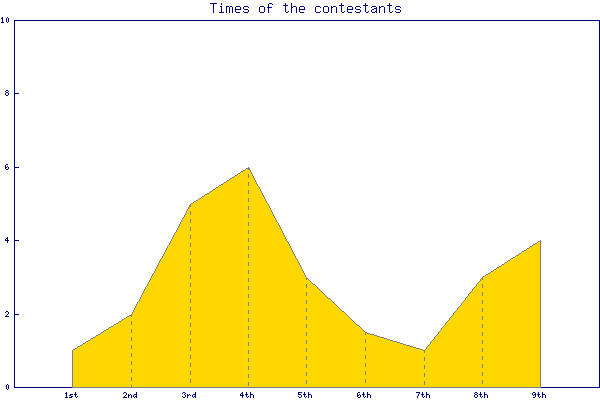
\includegraphics[width=0.9\textwidth]{image/3.png}
\end{center}
\end{figure}
\end{frame}

\begin{frame}[fragile] \frametitle{Points and Lines}
\begin{lstlisting}[language=perl_u,breaklines=true]
sub plotPng {    
    my $fileName = shift;
    @data = ( ["1st","2nd","3rd","4th","5th","6th","7th", "8th", "9th"],
              [    1,    2,    5,    6,    3,  1.5,    1,     3,     4]
            );
    my $mygraph = GD::Graph::points->new(600, 400);
    
    $mygraph->set (
        title         => "Times of the contestants",
        dclrs         =>  [ qw(gold red green) ],
    ) or warn $mygraph->error;

    my $myimage = $mygraph->linespoints(\@data) or warn $mygraph->error;
    
    open (IMG, '>' , $fileName);
    binmode IMG;
    print IMG $myimage->png;
    close (IMG);
}
\end{lstlisting}
\end{frame}

\begin{frame} \frametitle{Points and Lines - Output}
\begin{figure}[htbp]
\begin{center}
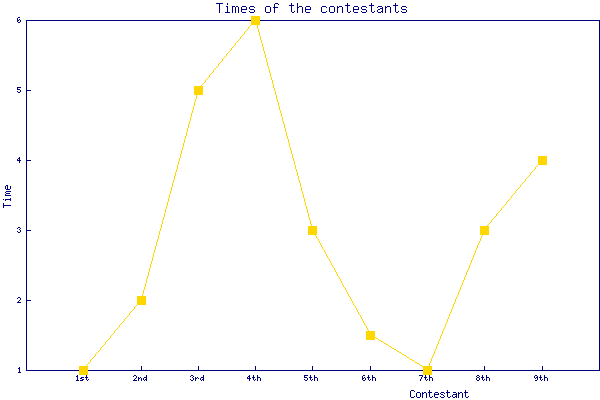
\includegraphics[width=0.9\textwidth]{image/4.png}
\end{center}
\end{figure}
\end{frame}

\begin{frame}[fragile] \frametitle{Examples of output formats}
\begin{lstlisting}[language=perl_u,breaklines=true]
print IMG $graph->plot(\@data)->gif;
print IMG $graph->plot(\@data)->png;
print IMG $graph->plot(\@data)->gd;
print IMG $graph->plot(\@data)->gd2;
\end{lstlisting}
\end{frame}

\begin{frame} \frametitle{Methods for all graphs}
\begin{description}
\item[$GD::Graph::chart->new(width,height)$] Create a new object $graph$ with optional width and heigth. Default $width$ = 400, default $height$ = 300. chart is either bars, lines, points, linespoints, area, mixed or pie.
\item[$graph->set\_text\_clr(colour name)$] Set the colour of the text. This will set the colour of the titles, labels, and axis labels to colour name. Also see the options $textclr$, $labelclr$ and $axislabelclr$.
\item[$graph->set\_title\_font(font specification)$] Set the font that will be used for the title of the chart.
\item[$graph->plot(data)$] Plot the chart, and return the GD::Image object.
\end{description}
\end{frame}

\begin{frame} \frametitle{Methods for all graphs - 2}
\begin{description}
\item[$graph->set(attrib1 => value1, attrib2 => value2 ...)$] Set chart options.
\item[$graph->get(attrib1, attrib2)$] Returns a list of the values of the attributes. In scalar context returns the value of the first attribute only.
\item[$graph->gd()$] Get the GD::Image object that is going to be used to draw on. You can do this either before or after calling the plot method, to do your own drawing.
\end{description}
\end{frame}

\begin{frame} \frametitle{Methods for all graphs - 3}
\begin{description}
\item[$graph->export\_format()$] Query the export format of the GD library in use. In scalar context, it returns 'gif', 'png' or undefined, which is sufficient for most people's use. In a list context, it returns a list of all the formats that are supported by the current version of GD. It can be called as a class or object method
\item[$graph->can\_do\_ttf()$]Returns true if the current GD library supports TrueType fonts, False otherwise. Can also be called as a class method or static method.
\end{description}
\end{frame}

\begin{frame} \frametitle{Options for graphs with axes}
\begin{description}
\item[$x\_label, y\_label$] The labels to be printed next to, or just below, the axes. Note that if you use the $two\_axes$ option that you need to use $y1\_label$ and $y2\_label$.
\item[$show\_values$] Set this to 1 to display the value of each data point above the point or bar itself.
\item[$values\_space$] Space to insert between the data point and the value to print. Default: 4.
\item[$values\_format$] How to format the values for display.
\end{description}
and many more\ldots
\end{frame}

\begin{frame}[fragile] \frametitle{Lines with $show\_values$}
\begin{lstlisting}[language=perl_u,breaklines=true]
    $mygraph->set (
        x_label => "Contestant",
        y_label => "Time",
        values_format => sub { return sprintf("\%d", shift); } , 
        values_space  => 10, 
        show_values  => 1,
        title         => "Times of the contestants",
        dclrs         =>  [ qw(gold red green) ]
    ) or warn $mygraph->error;
\end{lstlisting}
\end{frame}

\begin{frame}[fragile] \frametitle{Lines with $show\_values$}
\begin{figure}[htbp]
\begin{center}
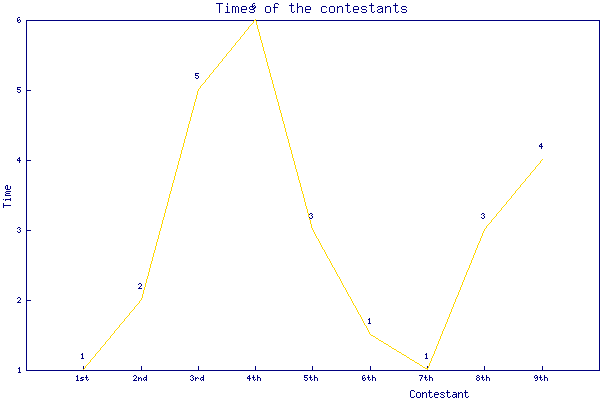
\includegraphics[width=0.9\textwidth]{image/linesNumbers.png}
\end{center}
\end{figure}
\end{frame}

\begin{frame}[fragile] \frametitle{Legends and multiple Y values}
\begin{lstlisting}[language=perl_u,breaklines=true]
    my @legend_keys = ("Nr of lines","Nr of comments");
    $mygraph->set_legend(@legend_keys);
    $mygraph->set(
        transparent   => 1,
        overwrite => 0,
        fgclr => black ,
        labelclr => black,
        axislabelclr => black,
        legendclr => black,
        valuesclr => black,
        textclr => black,
        transparent   => 1,
        overwrite => 0,
        bargroup_spacing => 10,
        show_values   => 1,
        values_format => sub { return sprintf("\%d", shift); } ,
        values_space  => 10,
        x_label       => $x_label,
        y_label       => $y_label,
        title         => $title,
        dclrs         =>  [ qw(gold red green) ],
    ) or warn $mygraph->error;
\end{lstlisting}
\end{frame}

\begin{frame}[fragile] \frametitle{Legends and multiple Y values - Output}
\begin{figure}[htbp]
\begin{center}
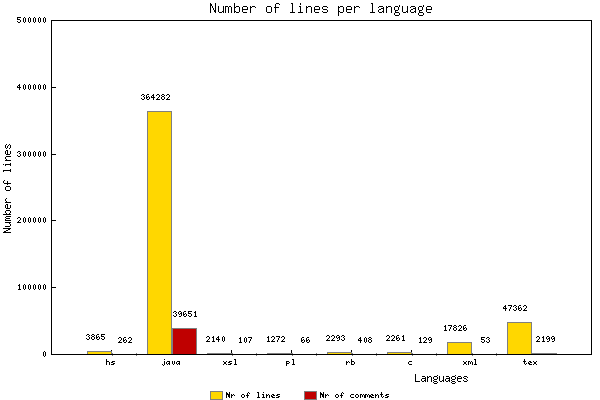
\includegraphics[width=0.9\textwidth]{image/msc_LinesPerLanguage.png}
\end{center}
\end{figure}
\end{frame}

\begin{frame}[fragile] \frametitle{Legends and multiple Y values 2 - Output}
\begin{figure}[htbp]
\begin{center}
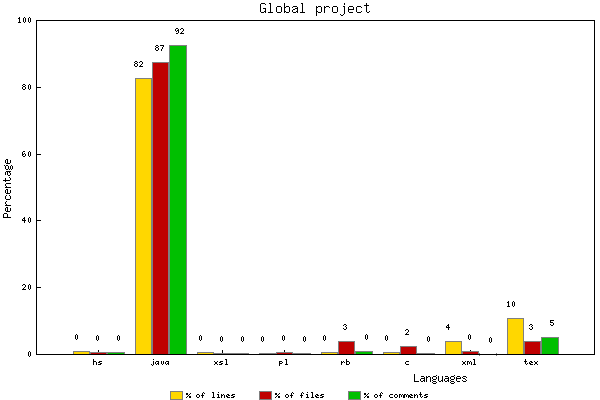
\includegraphics[width=0.9\textwidth]{image/msc_projectLanguages.png}
\end{center}
\end{figure}
\end{frame}

\begin{frame}[fragile] \frametitle{Overwrite bars}
\begin{lstlisting}[language=perl_u,breaklines=true]
    my @legend_keys = ("Nr of lines","Nr of comments");
    $mygraph->set_legend(@legend_keys);
    $mygraph->set(
        transparent   => 1,
        overwrite => 2,
        fgclr => black ,
        labelclr => black,
        axislabelclr => black,
        legendclr => black,
        valuesclr => black,
        textclr => black,
        transparent   => 1,
        overwrite => 0,
        bargroup_spacing => 10,
        show_values   => 1,
        values_format => sub { return sprintf("\%d", shift); } ,
        values_space  => 10,
        x_label       => $x_label,
        y_label       => $y_label,
        title         => $title,
        dclrs         =>  [ qw(gold red green) ],
    ) or warn $mygraph->error;
\end{lstlisting}
\end{frame}

\begin{frame}[fragile] \frametitle{Overwrite bars - Output}
\begin{figure}[htbp]
\begin{center}
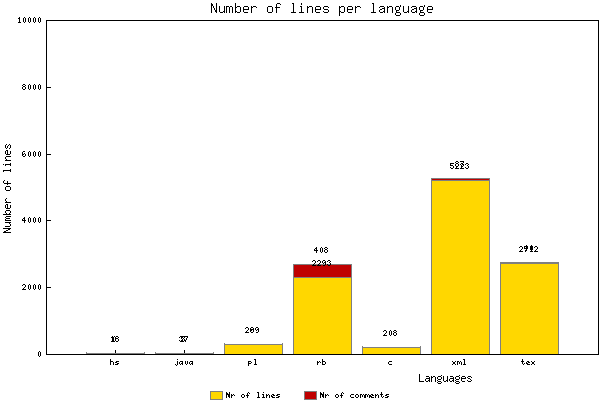
\includegraphics[width=0.9\textwidth]{image/image_LinesPerLanguage.png}
\end{center}
\end{figure}
\end{frame}
\section*{Perguntas}
\begin{frame} \frametitle{Perguntas}
\begin{center}\huge{?}\end{center}
\end{frame}

\end{document}

